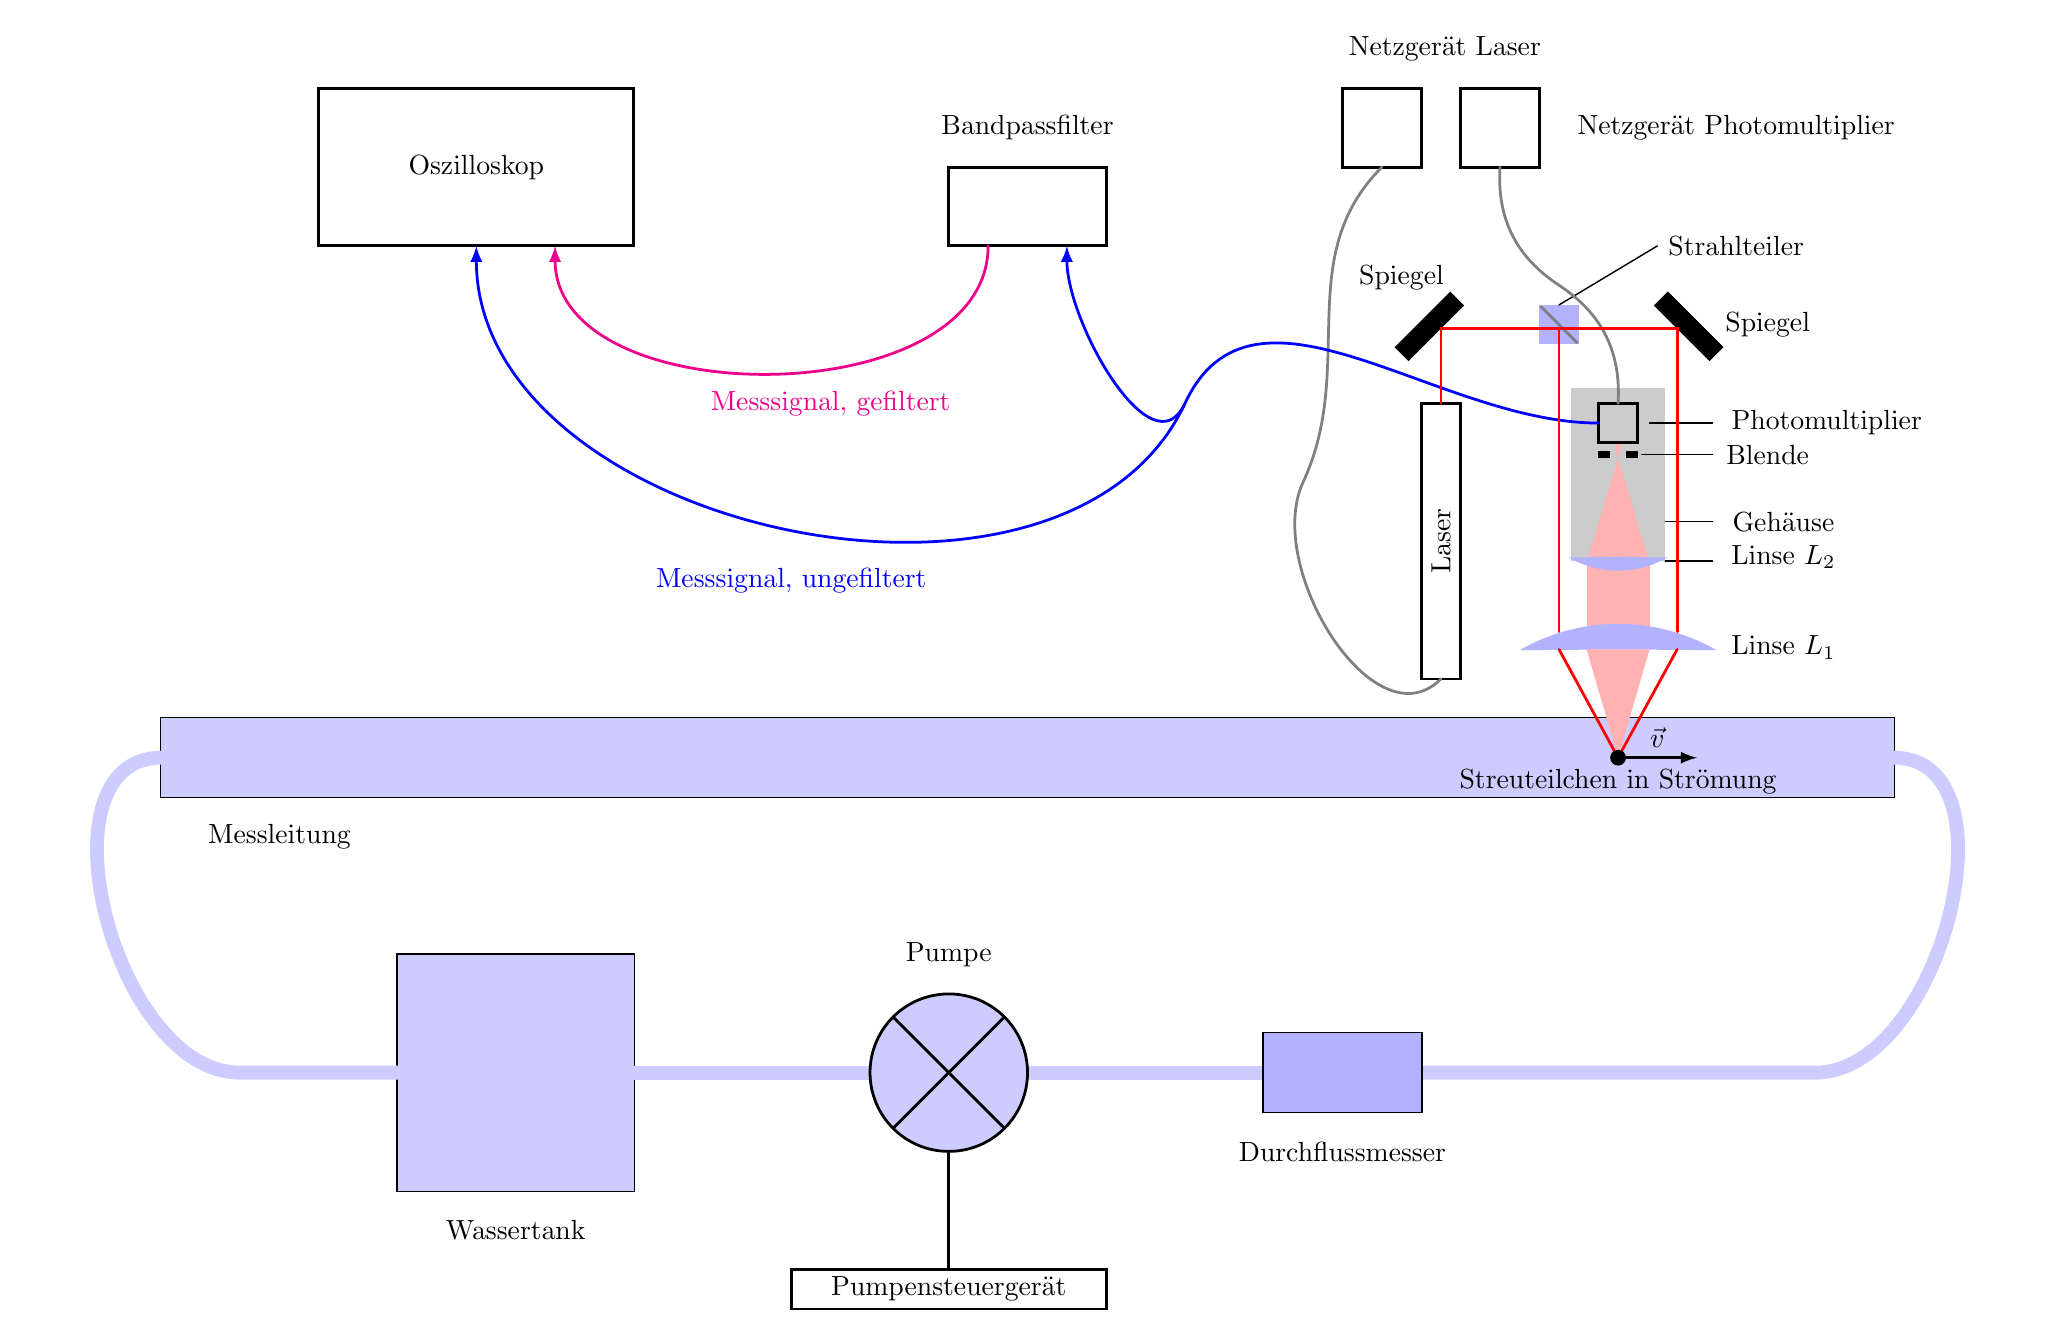
\begin{tikzpicture}
    \begin{scope}[x={(0mm,300mm)},y={(0mm,185mm)},line width=1pt,cap=round]
        % bounding box
        %\draw[black] (25mm,0mm) rectangle (275mm,175mm);

        % oscilloscope
        \draw[black] (60mm,160mm) rectangle (100mm,140mm);
        \node at (80mm,150mm) {Oszilloskop};

        % filter
        \draw[black] (140mm,150mm) rectangle (160mm,140mm);
        \node at (150mm,155mm) {Bandpassfilter};

        % PSU laser
        \draw[black] (190mm,160mm) rectangle (200mm,150mm);
        \node at (203mm,165mm) {Netzger\"at Laser};

        % PSU photomultiplier
        \draw[black] (205mm,160mm) rectangle (215mm,150mm);
        \node at (240mm,155mm) {Netzger\"at Photomultiplier};

        % measurement pipe
        \draw[black] (40mm,70mm) rectangle (260mm,80mm);
        \fill[blue!20] (40mm,70mm) rectangle (260mm,80mm);
        \node at (55mm,65mm) {Messleitung};

        % water tank
        \draw[black]   (70mm,20mm) rectangle (100mm,50mm);
        \fill[blue!20] (70mm,20mm) rectangle (100mm,50mm);
        \node at (85mm,15mm) {Wassertank};

        % pipe to tank
        \draw[-,blue!20,line width=5pt] (40mm,75mm)
            to [out=180,in=180] (50mm,35mm)
            to [out=0,in=180] (70mm,35mm);
        % tank to pump
        \draw[-,blue!20,line width=5pt] (100mm,35mm)
            to [out=180,in=180] (130mm,35mm);
        % pump to flow sensor
        \draw[-,blue!20,line width=5pt] (150mm,35mm)
            to (180mm,35mm);
        % flow sensor to pipe
        \draw[-,blue!20,line width=5pt] (200mm,35mm)
            to [out=0,in=180] (250mm,35mm)
            to [out=0,in=0] (260mm,75mm);

        % pump
        \fill[blue!20] (140mm,35mm) circle(10mm);
        \draw[black]   (140mm,35mm) circle(10mm);
        \draw[black,rotate around={-45:(140mm,35mm)}] (130mm,35mm) -- (150mm,35mm);
        \draw[black,rotate around={+45:(140mm,35mm)}] (130mm,35mm) -- (150mm,35mm);
        \node at (140mm,50mm) {Pumpe};

        % pump controller
        \draw[black] (140mm,25mm) -- (140mm,10mm);
        \draw[black]   (120mm,5mm) rectangle (160mm,10mm);
        \node at (140mm,7.5mm) {Pumpensteuerger\"at};


        % flow sensor
        \draw (180mm,30mm) rectangle (200mm,40mm);
        \fill[blue!30] (180mm,30mm) rectangle (200mm,40mm);
        \node at (190mm,25mm) {Durchflussmesser};

        % laser and cable
        \draw[black] (200mm,120mm) rectangle (205mm,85mm);
        \draw[black!50]        (195mm,150mm)
            to [out=-135,in=65] (185mm,110mm)
            to [out=-115,in=-135] (202.5mm,85mm);
        \node[rotate=90] at (202.5mm,102.5mm) {Laser};

        % mirror 1
        \fill[black,rotate around={45:(197.5mm,126.25mm)}] (197.5mm,125mm) rectangle (207.5mm,127.5mm);
        \node at (197.5mm,136mm) {Spiegel};

        % beam splitter
        \fill[blue!30]  (215mm,127.5mm) rectangle (220mm,132.5mm);
        \draw[black!50] (215.2mm,132.3mm) -- (219.8mm,127.7mm);
        \draw[black,line width=0.5pt] (217.5mm,132.5mm) -- (230mm,140mm);
        \node at (240mm,140mm) {Strahlteiler};

        % mirror 2
        \fill[black,rotate around={-45:(237.5mm,126.25mm)}] (227.5mm,125mm) rectangle (237.5mm,127.5mm);
        \node at (244mm,130mm) {Spiegel};

        % housing around detector and L2
        \fill[black!20] (219mm,122mm) rectangle (231mm,100mm);
        \draw[black,line width=0.5pt] (231mm,105mm) -- (237mm,105mm);
        \node at (246mm,105mm) {Geh\"ause};


        % dispersed light below lenses
        \fill[red!30] (221mm,90mm) rectangle (229mm,99.75mm);
        \fill[red!30] (221mm,99.75mm) -- (225mm,113mm) -- (229mm,99.75mm);
        \fill[red!30] (225mm,113mm) -- (224.5mm,115mm) -- (225.5mm,115mm);

        % detector and power cable and signal cables
        \draw[black] (222.5mm,120mm) rectangle (227.5mm,115mm);
        \draw[black!50] (210mm,150mm) to [bend right] (217.5mm,135mm) to [bend left] (225mm,120mm);
        \draw[-latex,blue] (222.5mm,117.5mm)
            to [out=180,in=65] (170mm,120mm)
            to [out=-115,in=-90] (155mm,140mm);
        \draw[-latex,blue] (170mm,120mm)
            to [out=-115,in=-90] (80mm,140mm);
        \draw[-latex,magenta] (145mm,140mm)
            to [out=-90,in=-90] (90mm,140mm);
        \node[magenta] at (125mm,120mm) {Messsignal, gefiltert};
        \node[blue] at (120mm,97.5mm) {Messsignal, ungefiltert};
        \node at (251.5mm,117.5mm) {Photomultiplier};
        \draw[black,line width=0.5pt] (229mm,117.5mm) -- (237mm,117.5mm);

        % aperture
        \fill[black] (222.5mm,114mm) rectangle (224mm,113mm);
        \fill[black] (226mm,114mm) rectangle (227.5mm,113mm);
        \draw[black,line width=0.5pt] (228mm,113.5mm) -- (237mm,113.5mm);
        \node at (244mm,113.5mm) {Blende};

        % lens L2
        \fill[blue!30] (225.25mm,100.5mm) -- (225mm,98.75mm) arc[start angle=-90,delta angle=-30,radius=12.5mm]  -- cycle;
        \fill[blue!30] (224.75mm,100.5mm) -- (225mm,98.75mm) arc[start angle=-90,delta angle=30,radius=12.5mm] -- cycle;
        \draw[black,line width=0.5pt] (231mm,100mm) -- (237mm,100mm);
        \node at (246mm,100.5mm) {Linse $L_2$};

        % lens L1
        \fill[blue!30] (224.75mm,88.75mm) -- (225mm,92mm) arc[start angle=90,delta angle=-30,radius=25mm] -- cycle;
        \fill[blue!30] (225.25mm,88.75mm) -- (225mm,92mm) arc[start angle=90,delta angle=30,radius=25mm]  -- cycle;
        \node at (246mm,89mm) {Linse $L_1$};

        % Laser beams
        % laser -> L1
        \draw[red] (202.5mm,120mm) -- (202.5mm,129.5mm) -- (217.5mm,129.5mm) -- (217.5mm,91mm);
        % L1 -> L1
        \draw[red] (217.5mm,88.75mm) -- (225mm,75mm) -- (232.5mm,88.75mm);
        % L1 -> beam splitter
        \draw[red] (232.5mm,91mm) -- (232.5mm,129.5mm) -- (217.5mm,129.5mm);
        % particle -> L1 (dispersion)
        \fill[red!30] (225mm,75mm) -- (229mm,88.75mm) -- (221mm,88.75mm);

        % particle
        \fill[black] (225mm,75mm) circle(1mm);
        \draw[-latex] (225mm,75mm) -- (235mm,75mm);
        \node at (230mm,77.5mm) {$\vec{v}$};
        \node at (225mm,72mm) {Streuteilchen in Str\"omung};

    \end{scope}
\end{tikzpicture}
